% Project 1 - EECS 499
% Authors: Shaun Howard and Matt Swartwout
\documentclass[conference]{IEEEtran} \usepackage[T1]{fontenc} \usepackage[backend=biber, style=ieee]{biblatex}
\addbibresource{report.bib} \usepackage[final]{microtype}

% *** GRAPHICS RELATED PACKAGES ***
%
\ifCLASSINFOpdf \usepackage[pdftex]{graphicx} % declare the path(s) where your graphic files are
  \graphicspath{{images/}} % and their extensions so you won't have to specify these with
  % every instance of \includegraphics
  \DeclareGraphicsExtensions{.jpeg,.png} \else % or other class option (dvipsone, dvipdf, if not using dvips). graphicx
  % will default to the driver specified in the system graphics.cfg if no
  % driver is specified.
  % \usepackage[dvips]{graphicx}
  % declare the path(s) where your graphic files are
  % \graphicspath{{../eps/}}
  % and their extensions so you won't have to specify these with
  % every instance of \includegraphics
  % \DeclareGraphicsExtensions{.eps}
\fi % graphicx was written by David Carlisle and Sebastian Rahtz. It is
% required if you want graphics, photos, etc. graphicx.sty is already
% installed on most LaTeX systems. The latest version and documentation
% can be obtained at:
% http://www.ctan.org/pkg/graphicx
% Another good source of documentation is "Using Imported Graphics in
% LaTeX2e" by Keith Reckdahl which can be found at:
% http://www.ctan.org/pkg/epslatex
%
% latex, and pdflatex in dvi mode, support graphics in encapsulated
% postscript (.eps) format. pdflatex in pdf mode supports graphics
% in .pdf, .jpeg, .png and .mps (metapost) formats. Users should ensure
% that all non-photo figures use a vector format (.eps, .pdf, .mps) and
% not a bitmapped formats (.jpeg, .png). The IEEE frowns on bitmapped formats
% which can result in "jaggedy"/blurry rendering of lines and letters as
% well as large increases in file sizes.
%
% You can find documentation about the pdfTeX application at:
% http://www.tug.org/applications/pdftex

% correct bad hyphenation here
\hyphenation{op-tical net-works semi-conduc-tor}


\begin{document}

% paper title
% Titles are generally capitalized except for words such as a, an, and, as,
% at, but, by, for, in, nor, of, on, or, the, to and up, which are usually
% not capitalized unless they are the first or last word of the title.
% Linebreaks \\ can be used within to get better formatting as desired.
% Do not put math or special symbols in the title.
\title{Distributed State Estimation in a 1-D World}


% author names and affiliations
% use a multiple column layout for up to three different
% affiliations
\author{ \IEEEauthorblockN{Shaun Howard \ \ Matt Swartwout} \IEEEauthorblockA{Electrical Engineering and Computer
Science Department\\ Case Western Reserve University\\ Cleveland, Ohio 44106\\ Email: \{smh150, mws85\}@case.edu} }

% make the title area
\maketitle

% As a general rule, do not put math, special symbols or citations
% in the abstract
\begin{abstract}
In this paper, we proposed the use of both an Extended Kalman Filter (EKF) and an Unscented Kalman
Filter (UKF) in order to determine the x-position of a single mobile robot (R) given multiple noisy sensor measurements.
Given a squadron of N robots in a one-dimensional environment, the x-position of robot R with noisy odometry data was
estimated via the sensor measurements of all N robots denoted S. Each robot in S monitored the true position of R via
a laser scan sensor in order to build a set of pose estimates for R. The resulting set of N pose estimates were fused
by means of a distributed network into either an EKF or UKF in order to accurately estimate the pose of R as it moved 
randomly between two networked robots in a one-dimensional simulator environment.

We demonstrated the usefulness of this state estimation procedure through a three robot simulation in Gazebo. We compared
the results of the distributed filter with a self-filter in this environment where R estimates its own position via
object detection and either an EKF or UKF. We simulated the use of each filter with varying speeds of R. We analysed and
compared filter results from each simulation in order to determine the reliability of each filter. Our simulation results
have revealed that the distributed EKF and UKF filters outperformed all other self-filter configurations in terms of accuracy 
without any additional parameter tuning.
\end{abstract}

\section{Introduction} \label{Introduction}
Networked cyber-physical systems have become more and more common in recent history. Traditionally, as the need for more
accuracy and precision has evolved with these systems the response has been to add more sensors. These sensors, when
combined together, e.g. a Kalman filter, can provide better state estimation than a single sensor alone. This is also
significantly cheaper than developing single sensors with extraordinary accuracy. However, as mobile robots and other
mobile autonomous technologies become more widespread the desire to decrease the cost and complexity of these devices
has increased. Adding more and more sensors to a single robot, while effective, is not cost-efficient for production and
leads to higher maintenance costs over the life of the robot.

One solution to this is distributed sensor networks. With recent developments in high-bandwith mobile radio
communications, sharing large amounts of sensor data over wireless networks has become much more feasible. Instead of
putting many sensors on one robot, many robots can use their one sensor and their observations of the other robots
around them to create a distributed state estimate for their companions.

Our system is based on the TurtleBot 2 platform and the Robot Operating System (ROS) \cite{ros_original}. The system is a simple 1-Dimensional exploration of the feasibility of distributed state estimation, using a mobile robot and two stationary landmarks as shown in figure 1. The mobile robot, using a LIDAR distance sensor, determines its position in the world by comparing itself to known stationary landmarks. At the same time, the known landmarks also use LIDAR to determine the mobile robots position. All of this data is then fused together in a Kalman filter, and compared to the output of a Kalman filter of just the robot's individual sensor, and also the ground truth of the simulator. Our simulations compare not only the "self" and "distributed" versions of the filter, but also examine the Extended Kalman Filter vs Unscented Kalman Filter and how they respond differently to the configurations. We also simulate the robot's motion at different speeds and compare the filter's performance when that is modified.

\begin{figure}
\label{pic1} 
\centering 
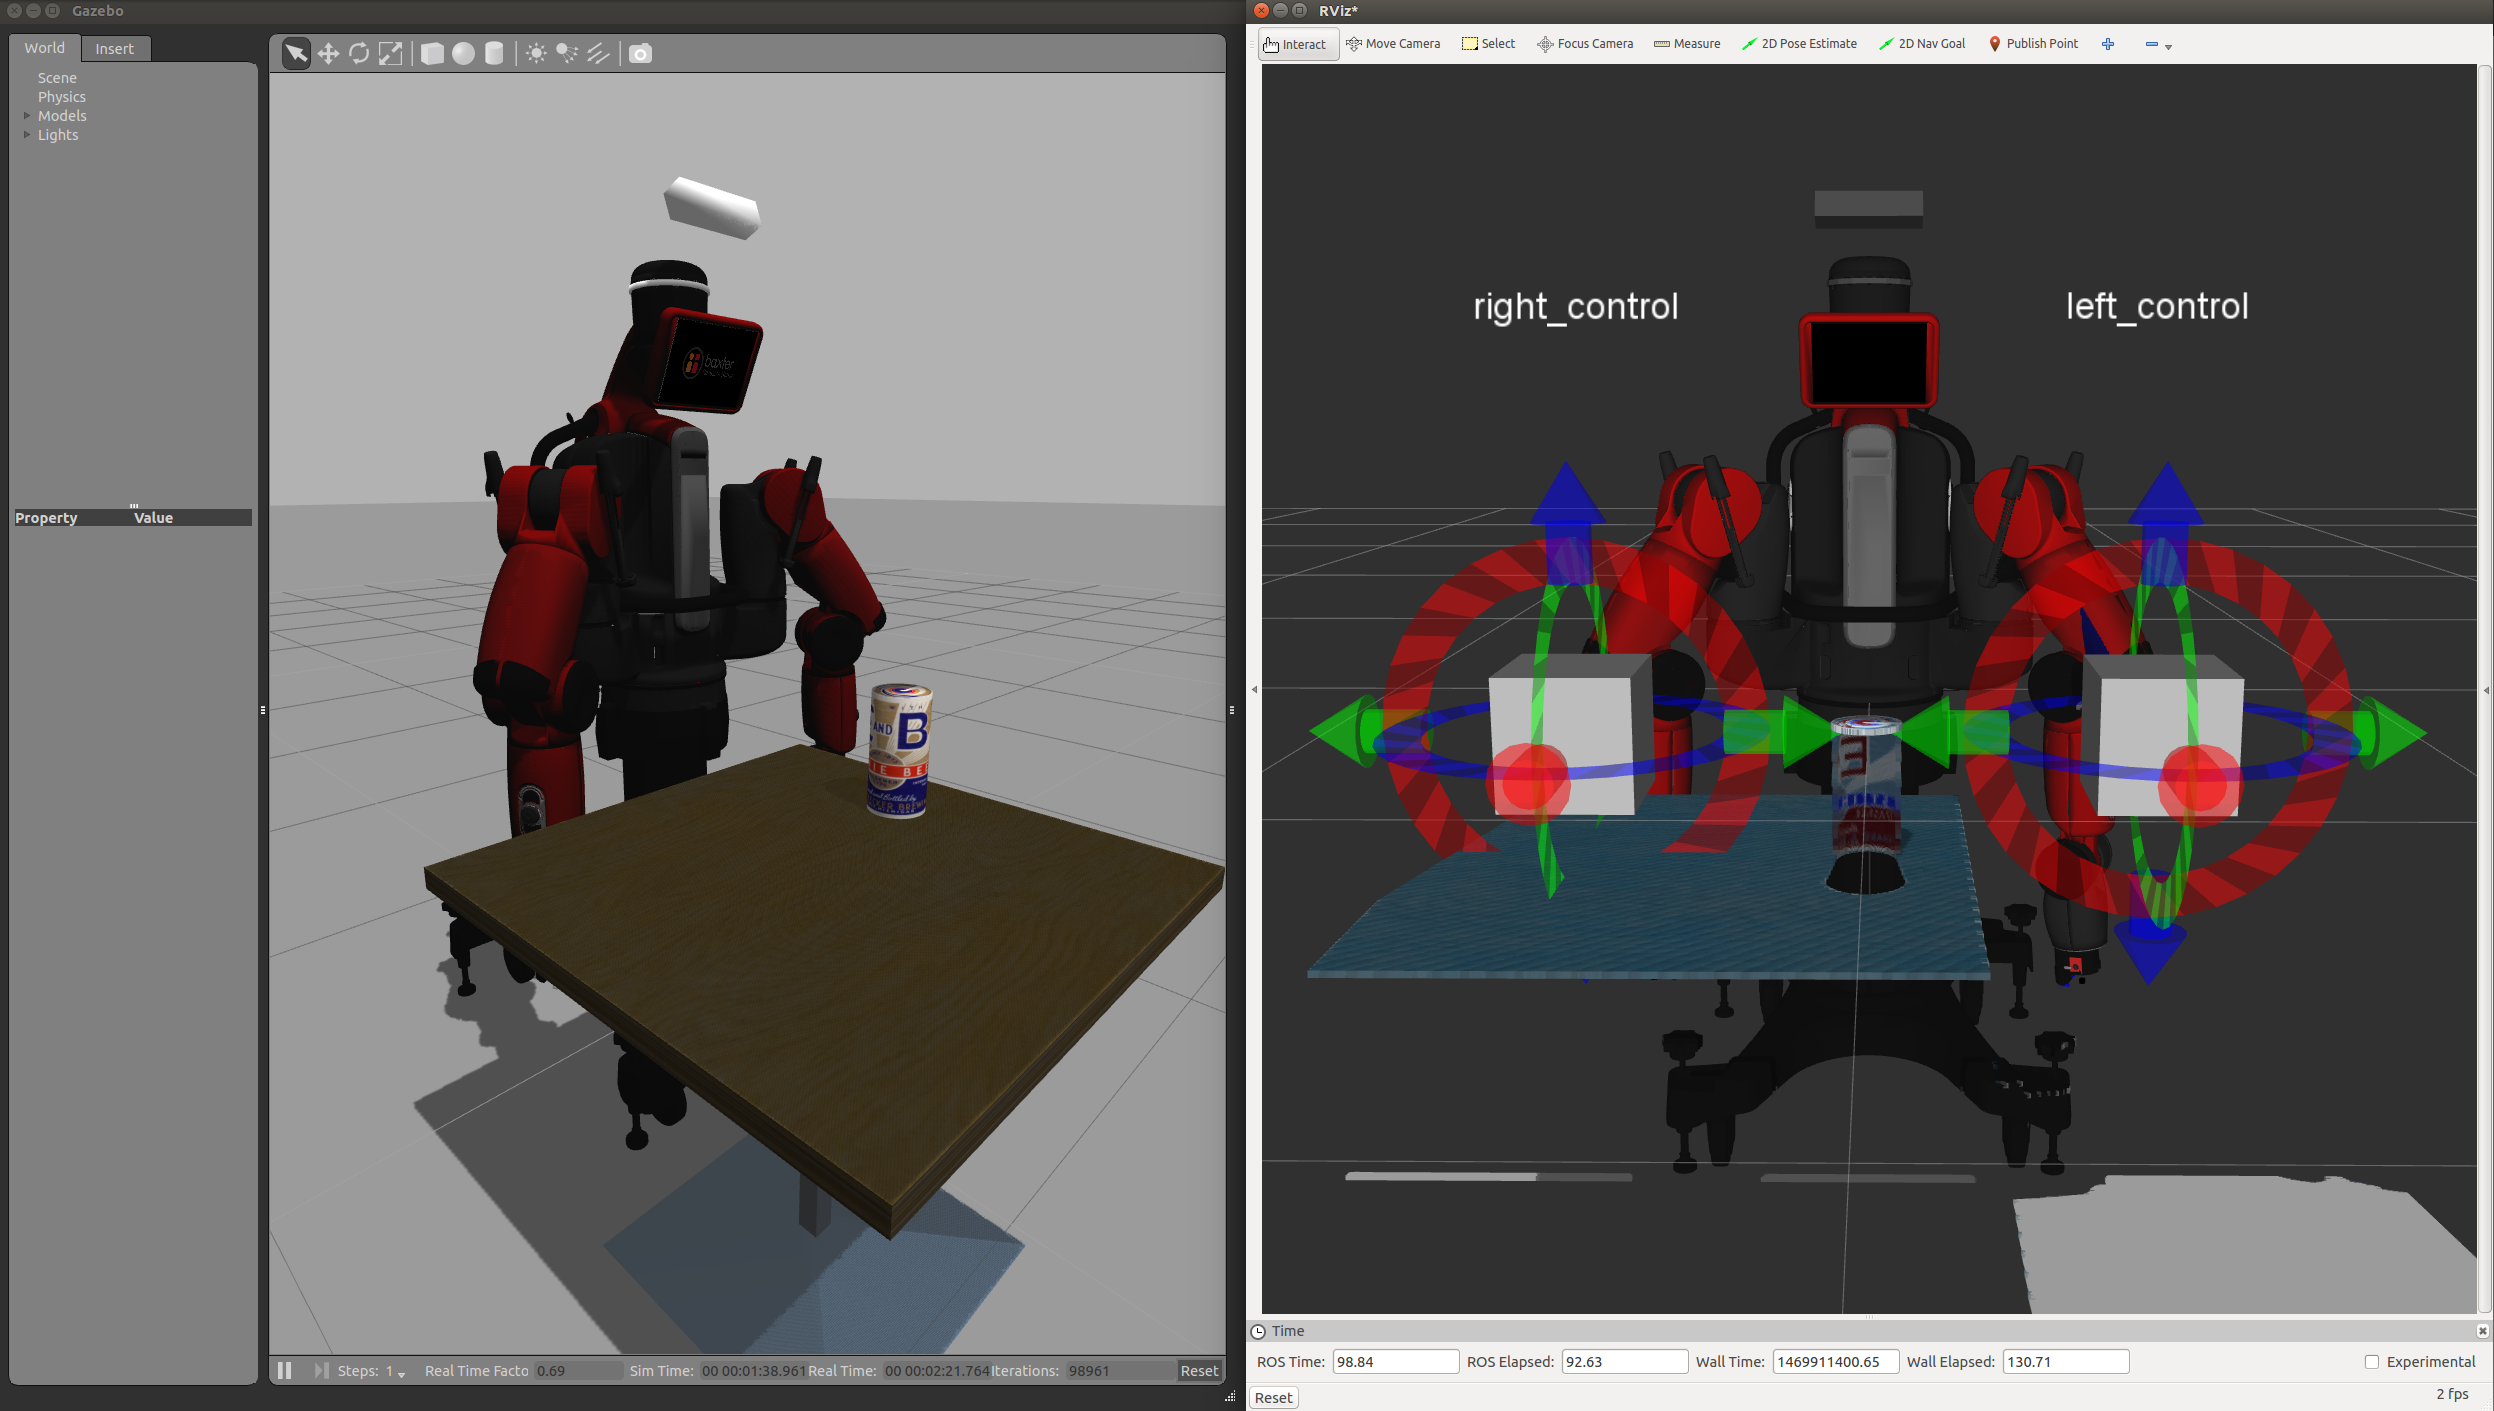
\includegraphics[width=0.49\textwidth]{sim1}
\caption{A squadron S of three TurtleBot 2's on a grid-based world attempt to estimate the position of R, the middle moving TurtleBot 2.}
\end{figure}

There are two primary contributions of this paper. First, we discuss related work. Second, we outline a system in ROS that implements a distributed sensor network 
between three robots and is easily scalable to an arbitrary number. Third, we statistically analyse and compare the position estimate results of the four different 
filter configurations given the egocentric first person perspective and distributed third-person perspective EKFs and UKFs.

\section{Related Work} \label{Related Work}
The idea behind our method was derived from the method proposed in \cite{bezzo2014attack}. Their method used an EKF to predict the position
of one terrorized robot given N-1 sensor measurements. The difference between methods is that our method analysed the
usage of an EKF and a UKF for estimating the position of a "lost" robot (R) given N positional (pose) estimates from both N-1 remote
sensors and one single sensor pose estimate from R's on-board laser scan sensor. Both filters show remarkable results in tracking 
the lost robot's position over time with the distributed filter, while the self-filter only works well with the EKF. Overall, 
the UKF beats the EKF in accuracy, and the distributed sensor network UKF worked best of all. Our simulation used three robots 
with one lost, uniformly randomly moving at a set speed between the two other robots in its local squadron. The two provided 
pose estimates and itself made an estimate based on landmark detection. A filter, either EKF or UKF, was used to estimate R's 
position. The experimental results prove our hypothesis that both the EKF and UKF work with an N-distributed sensor network.


\section{Problem Formulation} \label{Problem Formulation}
The concept of sensor fusion and combining multiple sensor readings within a single robot has been well shown. By
combining data from multiple sensors and feeding that information into an EKF or UKF, the total accuracy of the system
can be improved. Inherent noise in one sensor will propagate less into the final filter result, and the loss of a single or
multiple sensors theoretically should not result in catastrophic failure of the system given past proofs of the filter's success.

Our problem specification is created from the following core tenets:
\begin{enumerate} 
\item A finite 1-D system containing a mobile robot 
\item A physical landmark (e.g. stationary robot) at each end of the system
\item The mobile robot and landmarks are all equipped with a sensor that measures distance 
\item The mobile robot can move forwards and backwards, but cannot change its orientation (this obviates the need for a 
recognition system between the robot and landmarks)
\end{enumerate}

The core problems solved by our research methodology are the following:
\begin{enumerate}
\item Implementation of Extended and Unscented Kalman filters via the robot\_localization package \cite{robot_localization}
\item Creation of ROS system that simulates a TurtleBot 2 and the stationary landmarks in Gazebo \cite{gazebo}.
\item Creation of ROS node system for TurtleBot 2 that facilitates communication between a mobile robot and stationary 
landmarks as well as transforms and feeds those measurements into filter for pose estimation. 
\end{enumerate} 

\section{Methodology} \label{Methodology} As stated above, the project naturally divided itself into three main
problems. These three problems were the implementation of the Extended and Unscented Kalman filters, simulation of multiple
TurtleBot 2 robots in a Gazebo 1-D environment, and creation of a system of ROS nodes for the TurtleBot 2 to communicate with
the stationary landmarks and the filters.

\subsection{Sensor Measurements} \label{Sensor Measurements} Before describing our filter, we will describe how we
collected our distance measurements. Our measurements were taken by a simulated Microsoft Kinect camera, v1.0. We used
the depthimage\_to\_laserscan package \cite{depth_to_scan} to create a simulated LIDAR. Every scan (of ROS type
sensor\_msgs/LaserScan) received included a large number of ranges from different points in the scan. We used this
collection of ranges to create a single scan point that we then fed into the filter. We found that taking the median of
the scan ranges was far more accurate than the mean, so each filter input was the median of the scan ranges, with the
variance of the measurement being the variance of the entire group of measurements that was taken.

\subsection{Filter Implementation} \label{Filter Implementation} We chose to implement our filters using the previously
mentioned robot\_localization. We chose this package due to its ability to do sensor fusion of an arbitrary number of
sensors, because it was built for ROS, and because of the simple set up. Despite how easy it is, it allowed for complex configurations 
that gave us quite a bit of freedom without having to deal with the implementation details or tweaking many parameters.  

We applied both an Extended and Unscented Kalman filter with default parameters. We found that the default configuration 
parameters for both of the filters worked very well on the TurtleBot movement data. We applied these filter types in both
a self-sensor and a distributed sensor network fashion. The first filter we called the "self" filter, and
used only one distance measurement, taken by the moving robot's laser scan distance sensor for detecting an obstacle directly in front 
of it. The second filter we called the "distributed" filter. The distributed filter consumed three pose estimates and covariance matrices, 
two from the surrounding robots' laser scans and one from its own object detection. We realized that the covariance of these poses was just 
the variance since the world is one-dimensional, so this facilitated our experiment. Thus,  All measurements were fed to the filter as geometry\_msgs/PoseWithCovarianceStamped messages.

For both filters we set the two\_d\_mode parameter to true, because we did not care about any 3-dimensional motion. For the first
sensor measurement, we fused the x and y position and yaw into the final state estimate. Even though we assume a 1-D
system with no y movement possible, and also assume that no yaw rotations will ever be made, the filters do not support
a 1-D world so we had to include the y and yaw measurements. For the second and third sensor on the Distributed filter,
we fused only the x position.

We also set the differential parameter to true for all sensors. This makes the filter differentiate the absolute
position measurements received and input them as velocities rather than positions. This had two distinct advantages for
our system. First, we did not need to worry about transforming the poses from the reference frame of the landmark to the
reference frame of the mobile robot. Since we knew the starting position of the robot we did not need the absolute
position measurements. Second, this reduced the error from our measurement system. The system we used was a Kinect
camera, and we took a slice of points from its depth cloud and used this to simulate a LIDAR. Because of this, we were
not measuring a specific, known point on the robot. Instead, we measured many points and then took the median of those
points and represented that as the distance to the robot. By using the velocities rather than positions we mitigated
some of the error that may have come from the median point of the scan on the robot being in slightly different
positions from scan to scan. While error there may have existed, it would not lead to discrete jumps like the position
measurement would have.

We did not utilize any of the advanced parameters for either filter, and for the Unscented Kalman Filter we left the
alpha, beta, and kappa values at their defaults (0.001, 0, and 2, respectively). Once running, the filter nodes
published their topics via the standard ROS publish/subscribe system. We were able to view and record this data 
with rqt\_plot and rosbag commands.


\subsection{Gazebo Simulation} \label{Gazebo Simulation} Our simulation experiments were run in Gazebo with three
robots, two at fixed positions (stationary landmarks) and one moving randomly between the two (mobile robot). During
each experiment, the mobile robot moved randomly in the x-direction at a chosen experimental speed. Two speeds of 0.2
m/s and 0.4 m/s were chosen during experimentation for each filter type in order to determine the performance of filters
at various speeds in the one-dimensional environment.

The robot models used were the default TurtleBot 2 URDFs provided by the TurtleBot ROS package \cite{turtlebot}. The
robots were spawned into the world following the instructions laid out in the Gazebo Bringup Guide, with each robot
brought up inside of its own namespace to avoid conflicts. Each model by default includes an Xbox Kinect 3-D
camera used to detect landmarks in front of the robot using depth image information. The precision of the depth information
about surroundings directly in front of the robot is high. We used this depth information to create our own lidar 
sensor by using a specific angle of points directly in front of the robot. These points were used as a laser scan to emulate
a lidar 3-D laser scanner. The depth camera has its own frame which monitors the minimum and maximum range as well as position
of the camera in reference to the robot's base\textunderscore footprint\textunderscore self or base\textunderscore footprint\textunderscore
distributed frame used to distinguish where the robot was located in reference to the self and distributed sensors. A screenshot 
of R's RGB point cloud view from the camera\textunderscore frame is in figure 2.

\begin{figure}
\label{pic2} 
\centering 
\includegraphics[width=0.49\textwidth]{t2_camera_link}
\caption{A view in the perspective of the moving TurtleBot's camera\textunderscore link in reference to the camera\textunderscore rgb\textunderscore frame. 
The topic turtlebot2/odom is the simulator odometry pose.}
\end{figure}

The robots were spawned at Gazebo world coordinate (0,0), (2,0), and (4,0). The random motion of the mobile robot was
allowed between (1,0), and (3,0). These limits were chosen based on the Kinect's minimum range of 0.8 m and maximum range 
of 4 m. To create random motion, robot R sampled a random number uniformly between -1 and 1 and used that as its next increment
of movement in the x-direction. Direction was determined by the sign, with negative being backward and positive being forward. 
Then a boundary check was performed to validate that the final position after the move would be inside the movement bounds. 
If an invalid move was selected, the robot would wait until a new, valid positional movement amount was generated. If 
the goal was acceptable, R moved at the set experimental speed until it reached near the goal based on dead-reckoning. As R
moved, it's pose position and covariance were monitored by ROS via topics. The Gazebo simulator odometry was also tracked 
for the purpose of comparing the filtered odometry with the simulator odometry during analysis. This random motion repeated infinitely 
until either the simulation stopped or the robot drifted out of the parallel robot alignment setup which facilitated our experiment.

\subsection{Inter-Node Communication System} \label{Inter-Node Communication System} The communication system between
the ROS nodes was created very simply using the ROS publish/subscribe paradigm. Each of the TurtleBots constantly
processed the received LaserScans, as outlined in \ref{Sensor Measurements} and published them to a topic call
processed\_scan. The mobile robot then subscribed to these topics and created pose readings based on that sensor
measurement. These pose readings were then published on their own topic, which the filters were subscribed to. 
Finally, the filters output their total state estimation readings on a separate topic, which we were then able to
record, graph and analyse.

In essence, the use of ROS greatly simplified the networking of this system. Rather than having to work through the
intricacies of networking the robots together, we were able to create a system that is extensible to an arbitrary number
of robots and extremely resilient to failures, while also being incredibly simple to run and extend.

\section{Results} \label{Results} % discuss and display sim vs filtered odom using std dev error bars
\subsection{Data Acquisition and Analysis} \label{Data Acquisition and Analysis}
The ROS topics odometry pose messages echoed are 
recorded during the experiment with rosbag, converted to comma-separated value files, and analysed statistically with 
python and numpy. We visualize the results using matplotlib with a Matlab plotting interface via python. If one of the 
captured odometry topics is sampled at a higher frequency, a moving window average is used to estimate the data to match 
the other measurements one-to-one for analysis purposes. We take several statistics from the odometry data gathered per each experiment 
including mean, median, variance, standard deviation, standard error and root mean squared error. The 
experiments follow. 

\subsection{EKF Experiments} \label{EKF Experiments}
\subsubsection{R at 0.2 m/s} \label{EKF .2}
The first experiment runs the simulation with R moving at 0.2 m/s. Figure 3 shows a table of the result statistics for experiment 1 - EKF 
with R at 0.2 m/s. The data shows that the standard deviation, error and variance are higher in the distributed filter measurements than the 
self-filter measurements, but the self-filter has a higher root mean squared-error in accordance with the actual simulator odometry measurements than 
the distributed filter. From this fact, we can estimate that the distributed filter will perform better in this experiment than the self-filter.

\begin{figure}[!ht]
\label{pic3} 
\centering 
\includegraphics[width=0.49\textwidth]{ekf_2_table}
\caption{Experiment one statistics of self and distributed filter estimates against the exact simulator odometry measurements.} 
\end{figure}

Figure 4 displays a comparison of the predicted odometry measurements via the self EKF to the actual simulator 
odometry. As depicted in the image, the self-filter is not always within one standard deviation of the exact simulator 
odometry value. The self EKF tends to be inaccurate until it builds more confidence using its history of input values. We see early on it that it
is erroneous, especially with sharp direction changes, but it grows more reliable over time and along smooth intervals.

\begin{figure}

\centering 
\includegraphics[width=0.49\textwidth]{ekf_2speed_t2_self_filtered_odom_pos_err_graph}
\caption {A plot of the self-EKF position estimate along the simulator odometry curve over time 
reveals the inaccuracies of the ego-centric EKF in early stages but supports its convergence over time.
Error bars represent one standard deviation from the filtered value.}
\label{pic4} 
\end{figure}

\par
Figure 5 displays a comparison between the distributed EKF filter with R at 0.2 m/s and simulator odometry. The 
distributed filter tends to be within one standard deviation of the actual odometry values according to the graph. 
Given the tolerable error on position estimation in the distributed EKF, it clearly outperforms the self-filter 
in this experiment. Looking at the graph, we observe that the distributed filter handles early usage and sharp changes in direction well, 
and the simulator odometry measurement is always within one standard deviation from the filter estimate.

\begin{figure}
\centering 
\includegraphics[width=0.49\textwidth]{ekf_2speed_t2_dist_filtered_odom_pos_err_graph}
\caption {A plot of the distributed-EKF position estimate along the simulator odometry curve over time. It 
reveals the enhanced accuracy of the distributed filter over the ego-centric EKF. The distributed filter does not suffer 
from the inaccuracies in early usage and sharp direction change that the self-filter does.}
\label{pic5}
\end{figure}

\subsubsection{R at 0.4 m/s} \label{EKF .4}
The second experiment runs the simulation with R moving at 0.4 m/s. Figure 6 shows a table of the result statistics for 
experiment 2 - EKF with R at 0.4 m/s. The statistics reveal that the self-filter has a lower variance, standard deviation and error than the 
distributed filter, similar to the results shown in \ref{EKF .2}. However, the mean and median of the distributed filter position estimates closely 
agree with those values for the simulator odometry measurements. This hints that the self-filter is more precise with estimate generation, but it is 
sometimes prone to inaccuracies that throw it off, making it less reliable than the distributed filter at estimating position in general 
one-dimensional movement scenarios.

\begin{figure}[!ht]
\label{pic6} 
\centering 
\includegraphics[width=0.49\textwidth]{ekf_4_table}
\caption{Experiment two statistics of self and distributed filter estimates against the exact simulator odometry measurements.} 
\end{figure}

Figure 7 displays a comparison of the predicted odometry measurements via the self EKF to the actual simulator 
odometry. Similar to figure 4, the self filter is not always within one standard deviation of the exact simulator 
odometry value. The inaccuracies in the self-filter are upheld as we observe the erroneous drift that is corrected over time.

\begin{figure}
\centering 
\includegraphics[width=0.49\textwidth]{ekf_4speed_t2_self_filtered_pos_err_graph}
\caption {A second plot of the self-EKF position estimate along the simulator odometry curve over time 
upholds the inaccuracies of the ego-centric EKF in early stages as well as its response to sudden changes 
in movement.}
\label{pic7} 
\end{figure}

Figure 8 graphs the distributed EKF along the simulator odometry curve. The measurements are usually within one standard 
deviation of the actual values, but they reveal the inaccurate nature of the EKF in early stages of operation. These early readings 
are essentially sudden changes in the system that tend to create a brief drift which flows through the system until it is shortly 
corrected after multiple similar measurements from the landmark sensor. Support of the hypothesis in reference to the accuracy 
of the distributed Kalman filter over the self Kalman filter is slowly growing.

\begin{figure}
\centering 
\includegraphics[width=0.49\textwidth]{ekf_4speed_t2_dist_filtered_pos_err_graph}
\caption {A second plot of the distributed EKF position estimate along the simulator odometry curve over time 
upholds that the distributed EKF is usually more accurate than the self-filter but can also be prone to early drift on sudden 
perturbations.}
\label{pic8} 
\end{figure}

As we can see, the distributed EKF is prone to early drift via sudden perturbations in movement like the self-EKF but 
eventually corrects itself in little time. The rate at which it corrects itself is quicker than that of the self-filter. 
This is most likely due to the confidence the system has in the three sensor measurements over that it has in the single 
sensor measurement from R. This figure does however show more uncertainty than figure 5 due to higher speed. Perhaps some 
modifications to the EKF, e.g. using a UKF instead, will facilitate our proof of the hypothesis.

\subsection{UKF Experiments} \label{UKF Experiments}
\subsubsection{R at 0.2 m/s} \label{UKF .2}
The third experiment runs the simulation with R moving at 0.2 m/s. Figure 9 shows a table of the result statistics for experiment 3 - UKF 
with R at 0.2 m/s. The data consistently shows that the standard deviation, error and variance are higher by a small amount in 
the distributed filter measurements when compared with the self-filter measurements as with the EKF. However, 
the self-filter still has a higher root mean squared-error in accordance with the actual simulator odometry 
measurements than the distributed filter. From this fact, we can estimate that the distributed filter will 
again perform better in this experiment than the self-filter.

\begin{figure}[!ht]
\label{pic9} 
\centering 
\includegraphics[width=0.49\textwidth]{ukf_2_table}
\caption{Experiment three statistics of self and distributed filter estimates against the exact simulator odometry measurements.} 
\end{figure}

Figure 10 displays the self UKF filter at work with R at 0.2 m/s randomly moving back 
and forth. The results of the run are not as favourable as previously seen. The 
errors may be due to random ROS sensor errors or lack of parameter tuning. Perhaps 
the distributed UKF will perform better as predicted.

\begin{figure}
\centering 
\includegraphics[width=0.49\textwidth]{ukf_2speed_t2_self_filtered_pos_err_graph}
\caption {A plot of the self-UKF position estimate along the simulator odometry curve over time.}
\label{pic10} 
\end{figure}

The distributed UKF performs well in its experiment, as predicted. The distributed filter is consistently 
more inaccurate than the self-filter so far. One more experiment should be able to conclude the simulation process. 
Figure 11 graphs the results of this trial. 

\begin{figure}
\centering 
\includegraphics[width=0.49\textwidth]{ukf_2speed_t2_dist_filtered_pos_err_graph}
\caption {A plot of the distributed UKF position estimate along the simulator odometry curve over time.}
\label{pic11} 
\end{figure}

\subsubsection{R at 0.4 m/s} \label{UKF .4}
The fourth experiment runs the simulation with R moving at 0.4 m/s. Figure 12 shows a table of the result statistics for experiment 4 - UKF 
with R at 0.4 m/s. The data shows that the root mean squared error is high in the self filer as compared to the distributed filter. 
We find that the statistics for the distributed UKF pose estimates are very similar to the actual simulator 
odometry measurements. We can predict that the distributed filter will continue to dominate the self-filter in 
this experiment.

\begin{figure}[!ht]
\label{pic12} 
\centering 
\includegraphics[width=0.49\textwidth]{ukf_4_table}
\caption{Experiment four statistics of self and distributed filter estimates against the exact simulator odometry measurements.} 
\end{figure}

Figure 13 displays the results of running the self UKF at 0.4 m/s. The UKF does not 
appear to be very reliable for a single measurement at a higher speed. The measurements 
sometimes drift far off course and take a while to converge back to a reasonable 
confidence interval. Here we see that the self-UKF is no good for even a one-dimensional world with the default parameters.
In contrast, the distributed UKF in figure 14 unsurprisingly reveals that more sensor measurements lead to a greater
accuracy and precision in the filter as compared to the self-filter. 

\begin{figure}
\centering 
\includegraphics[width=0.49\textwidth]{ukf_4speed_1_t2_self_filtered_pos_err_graph}
\caption {A second plot of the self-UKF position estimate along the simulator 
odometry curve over time.}
\label{pic13} 
\end{figure}

\begin{figure}
\centering 
\includegraphics[width=0.49\textwidth]{ukf_4speed_1_t2_dist_filtered_pos_err_graph}
\caption {A second plot of the distributed UKF position estimate along the simulator odometry curve over time.}
\label{pic14} 
\end{figure}

Comparing both filtering approaches, we observe that the distributed filter almost always out-performs the self-filter 
with both filter types. Additionally, by no surprise we find that the UKF distributed filtering method out-performs the EKF distributed
filtering method. Overall, the results of our simulation support our hypothesis about the application of an EKF or UKF to accurately
estimate the position of a single mobile robot R via N sensor measurements given N robots networked in a distributed fashion in a 1-D environment. 
The self and distributed EKF work moderately well, but the UKF only works well with default parameters in a distributed system set up of at least 
two robots. Given more samples, the system was able to filter the data to predict output more accurately. We have shown that both the EKF 
and UKF work well in a distributed set up. Hopefully the idea of networking robots to share and predict accurate positional and state information will break new ground in the world of distributed and intelligent robotics network systems given the results of our distributed sensor network state prediction
system.

\section{Conclusion} \label{Conclusion} 
From the results of these experiments, we can form multiple conclusions. The first and most important observation is that a distributed sensor network consistently 
out-performs the self sensor system. This is not surprising. By adding more sensor data, the filters are able to create more accurate state estimates. Second, we 
must examine our result that the EKF out-performed the UKF in the single sensor configuration. We believe this is not an important result for two reasons. First, the 
main advantage of a UKF over an EKF is a non-linear system. However, our mobile robot moved at constant velocity in one dimension, greatly diminishing the 
advantages of the UKF. Further, a mobile robot with one sensor will never be a realistic model. Any production robot will have more than one sensor on-board for 
localization, so we believe that fusion of multiple sensors per robot would create an even better distributed system with direct increase and no real overhead if 
the robots are already available. We know that this research is extensible further than this very specific and one-dimensional instance based on class research, and 
we have shown that the UKF will almost always be the best choice of Kalman filter for distributed sensor fusion pose estimation.

We have shown that the distributed system for multiple sensor measurements is a viable option and may increase robot reliability. The method is not top-heavy, 
for the distributed networking system is very fast in transmission and computation because it is modelled after an individual mobile robot sensor fusion system as 
in \cite{bezzo2014attack}. Our additional contribution is to abstract away the state estimation system to ROS nodes while the robots run independently of each other. If employed in 
a real robot network, an external ROS node server could monitor each of the robots individually and handle all networking details based on preconfigured files. 
This method will not increase cost as dramatically as adding more sensors to an individual robot would. We believe and hope to suggest that distributed robot sensor 
networks are a viable means of robot communication for driving cooperation and positional information estimation based on individual viewpoints. This filtering 
technique could be applied for position estimation if on-board odometry sensors are very noise or if the navigation system is 
compromised. A secure state prediction squadron employing this research could be used in autonomous vehicles, transport, defense, flight, 
industry, and agriculture. As networked mobile robots become more and more prevalent, the cost and 
reliability of a distributed sensor network system will continue to decrease, effectively making easy-to-network robots more maintainable and manageable for 
businesses and people to use everyday.

\subsection{Future Work}
There are a number of future possibilities for expanding upon this work and verifying the results we found. The first is to increase the realism of the simulation. We chose a 1-D, constant velocity, single sensor per robot simulation because it allowed for simple verification of our hypotheses. However this is not a realistic use case for a mobile robot. We would like to see the simulation expanded to two dimensions, varying velocities, and $\geq 3$ sensors per robot. Additionally, the Gazebo environment contains practically zero sensor noise. Expanding the simulation to include realistic noise would give a better indication of the EKF vs. UKF performance and also what sort of accuracy can be expected in a real world use case.

Further, there is a large opportunity for research in the area of mobile robot security. \cite{bezzo2014attack}, \cite{fawzi2011secure}, and \cite{mo2014resilient} all demonstrate work with Kalman Filters that reduces the impact of sensor attacks on the final state estimate. Further, all of these focus on a single robot with multiple sensors. In the case of mobile robots and real world use however, there is very little guarantee that sensors will not be tampered with on a robot. And if an attacker has physical access to the entire robot, they could realistically attack every sensor. Thus, a distributed sensor network could provide a robust system resilient to attacks against one or multiple robot's sensors. 

\printbibliography
\end{document}